\section* {3.1}

\subsection{Постановка задачи}
Используя таблицу значений $Y_i$  функции $y=f(x)$, вычисленных в точках   $X_i, i=0,..3$  построить интерполяционные многочлены Лагранжа и Ньютона, проходящие через точки $\{X_i,Y_i \}$ .  Вычислить значение погрешности интерполяции в точке $X^*$. 

{\bfseries Вариант:} 12

$y=sin(x)+x, a) X_i= 0, \pi/6, 2\pi/6, 3\pi/6;  б)X_i= 0, \pi/6, \pi/4, \pi/2; X^* = 1.0$
%\pagebreak

\subsection{Результаты работы}
\begin{figure}[h!]
\centering
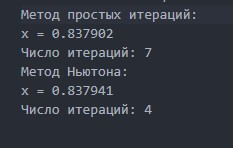
\includegraphics[width=12cm, height=6.5cm]{img1}
\caption{Вывод программы в консоли}
\end{figure}
\pagebreak
% \vfill


\subsection{Исходный код}
Файл с первым заданием третьей лабораторной работы:
\lstinputlisting{include/task1.cpp}
\pagebreak

\section* {3.2}

\subsection{Постановка задачи}
Построить кубический сплайн для функции, заданной в узлах интерполяции, предполагая, что сплайн имеет нулевую кривизну при $x=x_0$  и $x=x_4$. Вычислить значение функции в точке $x=X^*$. 

{\bfseries Вариант:} 12
\begin{figure}[h!]
$X_i=0.8$
\centering
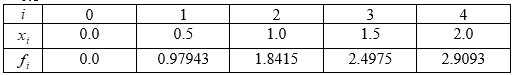
\includegraphics[width=15cm, height=4cm]{img2_0}
\caption{Условие}
\end{figure}
%\pagebreak

\subsection{Результаты работы}
\begin{figure}[h!]
\centering
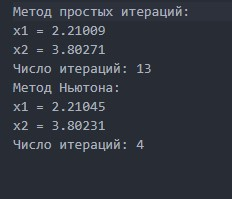
\includegraphics[width=15cm, height=3cm]{img2}
\caption{Вывод программы в консоли}
\end{figure}
\pagebreak

\subsection{Исходный код}
Файл со вторым заданием третьей лабораторной работы:
\lstinputlisting{include/task2.cpp}
\pagebreak

\section* {3.3}

\subsection{Постановка задачи}
Для таблично заданной функции путем решения нормальной системы МНК найти приближающие многочлены a) 1-ой  и б) 2-ой степени. Для каждого из приближающих многочленов вычислить сумму квадратов ошибок. Построить графики приближаемой функции и приближающих многочленов.

{\bfseries Вариант:} 12
\begin{figure}[h!]
\centering
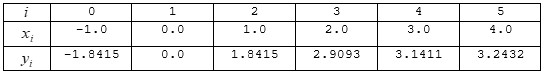
\includegraphics[width=15cm, height=4cm]{img3_0}
\caption{Условия}
\end{figure}
%\pagebreak

\subsection{Результаты работы}
\begin{figure}[h!]
\centering
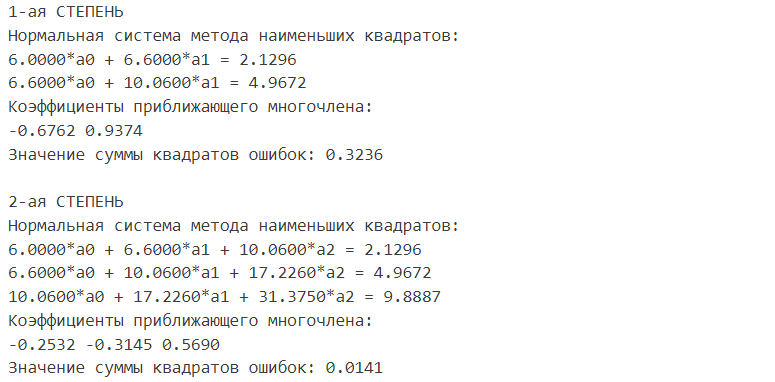
\includegraphics[width=15cm, height=4cm]{img3}
\caption{Вывод программы в консоли}
\end{figure}
\pagebreak

\subsection{Исходный код}
Файл с третьим заданием третьей лабораторной работы:
\lstinputlisting{include/task3.cpp}
\pagebreak

\section* {3.4}

\subsection{Постановка задачи}
Вычислить первую и вторую производную от таблично заданной функции $y_i=f(x_i), i=0,1,2,3,4$  в точке $x=X_i$.   

{\bfseries Вариант:} 12
$X^*=0.2$

\begin{figure}[h!]
\centering
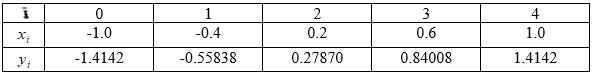
\includegraphics[width=15cm, height=2cm]{img4_0}
\caption{Условия}
\end{figure}
%\pagebreak

\subsection{Результаты работы}
\begin{figure}[h!]
\centering
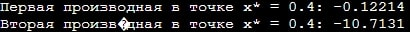
\includegraphics[width=10cm, height=2cm]{img4}
\caption{Вывод программы в консоли}
\end{figure}
\pagebreak

\subsection{Исходный код}
Файл с четвертым заданием третьей лабораторной работы:
\lstinputlisting{include/task4.cpp}
\pagebreak
\section* {3.5}

\subsection{Постановка задачи}
Вычислить определенный интеграл $\int\limits_{X_0}^{X_1} y dx$  , методами прямоугольников, трапеций, Симпсона с шагами $h_1,h_2$. Оценить погрешность вычислений, используя  Метод Рунге-Ромберга: 

{\bfseries Вариант:} 12\\
$y= x/(x^3+8)$
$X_0=-1, X_k=1, h_1=0.5, h_2=0.25$

\subsection{Результаты работы}
\begin{figure}[h!]
\centering
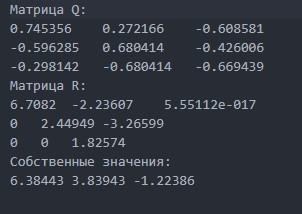
\includegraphics[width=10cm, height=10cm]{img5}
\caption{Вывод программы в консоли}
\end{figure}
\pagebreak

\subsection{Исходный код}
Файл с пятым заданием третьей лабораторной работы:
\lstinputlisting{include/task5.cpp}